\documentclass[tcc,capa]{texufpel}

\usepackage[utf8x]{inputenc} % acentuacao
\usepackage{graphicx} % para inserir figuras
%\usepackage[latin1]{inputenc}
\usepackage{ textcomp }
\hypersetup{
    hidelinks, % Remove colora��o e caixas
    unicode=true,   %Permite acentua��o no bookmark
    linktoc=all %Habilita link no nome e p�gina do sum�rio
}
\usepackage{ upgreek }
\usepackage{amsfonts}
\usepackage[linguistics]{forest}
\unidade{Centro de Desenvolvimento Tecnológico}
\curso{Ciência da Computação}
\nomecurso{Bacharelado em Ciência da Computação}
\titulocurso{Bacharel em Ciência da Computação}

\title{ExMOD-GM: Extension for Measurement Operations on the D-GM Enviromment}

\author{Silveira Neto}{Julio Machado da Silveira Neto}
\advisor[Prof.~Dr.]{Reiser}{Renata Hax Sander}
\coadvisor[Prof.~Dr.]{Pilla}{Maurício  Lima}

%Palavras-chave em PT_BR
\keyword{palavrachave-um}
\keyword{palavrachave-dois}
\keyword{palavrachave-tres}
\keyword{palavrachave-quatro}

%Palavras-chave em EN_US
\keywordeng{keyword-one}
\keywordeng{keyword-two}
\keywordeng{keyword-three}
\keywordeng{keyword-four}

\begin{document}

%\renewcommand{\advisorname}{Orientadora}           %descomente caso tenhas orientadora
%\renewcommand{\coadvisorname}{Coorientadora}      %descomente caso tenhas coorientadora

\maketitle 

\sloppy

\fichacatalografica

\folhadeaprovacao

%Opcional
\begin{dedicatoria}

\end{dedicatoria}

%Opcional
\begin{agradecimentos}

\end{agradecimentos}

%Opcional
\begin{epigrafe}

  {\sc --- Fulano de Tal}
\end{epigrafe}

%Resumo em Portugues (no maximo 500 palavras)
\begin{abstract}

\end{abstract}

\begin{englishabstract}%
  {ExMOD-GM: Extension for Measurement Operations on the D-GM Enviromment}%

  

  

\end{englishabstract}

%Lista de Figuras
\listoffigures

%Lista de Tabelas
\listoftables

%lista de abreviaturas e siglas
\begin{listofabbrv}{SPMD}
    \item[IEEE] Institute of Electrical and Electronics Engineers
        \item[CQ] Computação Quântica
        \item[ABNT] Associação Brasileira de Normas Técnicas
        \item[MQ] Mecânica Quântica
        \item[PEs] Processos Elementares
        \item[CF] Conjuntos Fuzzy
        \item[qGM] Quantum Geometric Machine Model
        \item[VPE-qGM] Visual Programming Environment for the qGM
        \item[qubit] Bit Quântico 
        \item[PE] Processo Elementar
\end{listofabbrv}

%Sumario
\tableofcontents

\chapter{Introdução}
Neste trabalho é realizada a concepção do  projeto \emph{ExMOD-GM: Extension for Measurement Operations on the D-GM Enviromment}, que visa o desenvolvimento de uma extensão no ambiente VPE-qGM \cite{maron:2013:ccgrid} permitindo que seja feita medidas simultâneas nos qubits dos circuitos quânticos, através do estudo, análise e implementação de outras medidas quânticas apresentadas no trabalho.

A Computação Quântica (CQ) é um paradigma fundamentado nos fenômenos
da mecânica quântica \cite{chuang00a}. A aplicação destes conceitos na computação permite alcançar um desempenho que  chega a ser exponencialmente maior do que computadores clássicos. Apesar de todos os esforços, vários desafios técnicos, como o aumento exponencial do uso de memória, limitam os sistemas atuais à apenas alguns bits quânticos \cite{steeb2011problems}.

Devido à indisponibilidade de hardware quântico, o estudo e desenvolvimento de aplicaçõess na CQ usualmente é feito estritamente pela especificação matemática das
computações ou por meio de ferramentas de simulação. Este último caracteriza a abordagem mais prática, entretanto, a complexidade computacional associada á simulação de
sistemas quânticos a partir de computadores clássicos limita o tamanho dos sistemas que
podem ser simulados.


\begin{quote}

\end{quote}
  




\chapter{Computação Quântica}



%revisão bibliográfica
%--computação quantica
Este capítulo apresenta conceitos da Computação Quântica [CQ] que é um paradigma computacional com foco no desenvolvimento de computadores mais rápidos do que os computadores clássicos, esse desempenho se dá no fato de que a CQ está baseada nos postulados da Mecânica Quântica[MQ]. Nas próximas sessões serão apresentados os fundamentos da MQ que a CQ utiliza.
%~falar onde esse desempenho vai ser aplicado
%--brevemente mecanica quantica
\section{Mecânica Quântica}
Como dito anteriormente, a MQ estabelece os princípios físicos para o desenvolvimento de computadores quânticos. As definições e propriedades da MQ são apresentadas em formas de postulados, pois os circuitos quânticos devem respeitar matematicamente as formulações físicas, de modo que as propriedades físicas da MQ sejam utilizadas pelas CQ.
Na física clássica, um estado pode assumir apenas um valor(0 ou 1), podemos dar como exemplo o spin de um elétron, que pode ser positivo ou negativo. Diferente disso, na MQ um estado pode assumir os dois valores simultãneamente(0 e 1), ou seja, o spin do elétron pode ser positivo e negativo ao mesmo tempo. Essa propriedade é chamada de superposição de estados e é uma das mais expressivas a MQ \cite{MARON10}.
A MQ interpreta o princípio da dualidade onda-partícula, comportamento apresentado por elementos sub-atômicos, mais precisamente o elétron:
\begin{itemize}
    \item Corpuscular: gira em torno do núcleo atômico e possui uma trajetória bem definida.
    \item Ondulatório: comporta-se como uma onda eletromagnética com superposição de fases.
\end{itemize}
Esse padrão de comportamento representa a explicação física da superposição existente na descrição da informação quãntica. Desse padrão deriva-se o princípio da incerteza de Heisenberg \cite{courteille2014mecanica}. Este define que durante o processo de mensuração de um estado quãntico ocorre a alteração do mesmo, e depois dessa modificação, o estado deixa de ser quântico. Isso ocorre devido a um sistema fechado não ser sujeito a perda de energia, quando aplica-se o processo de mensuração o sistema é violado desequilibrando o sistema, ocorrendo assim a perda de energia. O Experimento da Fenda Dupla demonstra que uma partícula quântica é expressa por uma função de onda que representa a variação de estados possíveis para um sistema.
Existe também o princípio do emaranhamento entre duas partículas. Dois ou mais objetos podem estar conectados de tal modo que a face de um dos objetos não pode ser analisada adequadamente sem que a outra face do objeto não seja afetada, mesmo que ambos não estejam localizados no mesmo espaço dimensional(tele transporte quântico) \cite{chuang00a}. 
Desse modo, temos que a MQ é percursora da CQ cusjas especificações derivam matemáticas que permitem expressar a relação de corretude entre o meio físico e o meio computacional. Nas próximas sessões serão apresentados os postulados mais relevantes da MQ para a realização deste projeto.
%postulados

\subsection{Primeiro Postulado: Princípio da Superposição}

O estado de um sistema é descrito por uma função complexa $\psi$ das coordenadas de todas as partículas do sistema e do tempo. Esta função designada por função de onda, contém toda a informação que se pode obter sobre o sistema. Postula-se ainda que $\psi$ admite apenas uma interpretação, é contínua e quadraticamente integrável.
Assim, qualquer sistema físico isolado está associado a um espaço vetorial complexo com um produto interno, espaço de Hilbert. A descrição se dá pelo seu vetor unitário no espaço de estados. \cite{loss}.
\begin{itemize}
    \item Espaço de Hilbert: O conjunto de funções unívocas, contínuas quadraticamente integráveis de n variáveis, com adição usual de funções, a multiplicação usual por um escalar e o produto interno:
    
\centering    $\langle\varphi((\vec{q})|\varphi(\vec{q})\rangle=\int \varphi * (\vec{q})\varphi(\vec{q})dt $
    
    onde $dt$=$\prod dq_i$ forma um espaço de Hilbert, espaço vetorial normado de dimensão infinita\cite{loss}. 
    Expondo matematicamente, pode-se definir um espaço de Hilbert $H (C^m)$, da seguinte forma, se $H$ for um espaço vetorial complexo como produto interno quivalente ao espaço de Banach(espaço vetorial normado completo) com $norma^1$ derivada do produto interno \cite{biezuner2009notas}.
\end{itemize}

\subsection{Espaço de Estados}
Do primeiro postulado definimos a representação do espaço de estados de um sistema quântico e suas propriedades físicas de existência. Logo, a representação em um sistema físico de dois estados se dá por um bit, já um sistema quântico com a mesma definição em relação ao espaço de estados pode ser representado por um q-bit(bit quântico).  Dessa forma representamos as seguintes definições\cite{maron:2013:ccgrid}, \cite{Schmalfuss14}:
\begin{itemize}
    \item Qubit: É a unidadde básica de informação, composto por um vetor unitário e bidimensional com componentes complexos, genericamente representados, na notação de Dirac, equacionada como $|\psi\rangle= \alpha|0\rangle + \beta|1\rangle$. Nesta equação $\alpha$ e $\beta$ são números complexos correspondentes as amplitudes dos respectivos estados.
    \item Normalização: Condição de existência que um estado $\phi$ deve satisfazer, assim, $\phi$ deve ser um vetor unitário restrido a um espaço normado $|\alpha|^2 + |\beta|^2=1$ 
    \item Superposição: Um qubit pode estar em superposição de estados clássicos, isto é, o estado $|\phi\rangle$ pode poussir em seu interior $|0\rangle$ e $|1\rangle$ simultaneamente. 
\end{itemize}

A representação geométrica de um qubit se dá através da esfera de Bloch, ilustrada na figura \ref{fig:Bloch}, define geometricamente o espaço ortogonal onde as fases de um qubit estão representadas(rotação em direção ao spin)~\cite{chuang00a}, desse modo, através de transformações matemáticas podemos analisar as possibilidades de valoração e fase para um estado. Para a representação geométrica de múltiplos qubits utiliza-se a notação n-esferas, onde n representa as dimensões, (CASTRO, 2004). PEGAR REFERENCIA


\begin{figure}[ht]
    \centering
    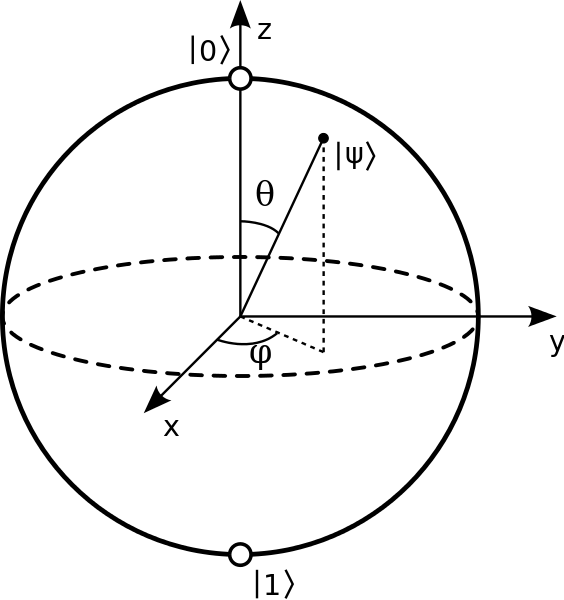
\includegraphics[width=.2\textwidth]{imagens/blochSphere.png}
    \caption{Esfera de Bloch}
    \label{fig:Bloch}
\end{figure}

Como temos a seguinte condição de normalização  $|\alpha|^2 + |\beta|^2=1$, logo, podemos representar os possíveis valores de um qubit na esfera de Bloch de acordo com a seguinte equação:
\begin{equation}
    |\psi\rangle= e^i^\gamma(cos\frac{\uptheta}{2}|0\rangle + e^i^\phi sen\frac{\uptheta}{2}|1\rangle )
    \label{eqBloch}
\end{equation}

Analisando a projeção que a~\ref{eqBloch} nos dá, o fator $e^i^\gamma$ pode ser desconsiderado, pois não é um valor observável($|e^i^\gamma|=1$). Os números $\uptheta$, $\phi$ e $\gamma$ $\in$ $\mathbb{R}$,  com $\uptheta$ e $\phi$ sendo um ponto representado por um raio unitário. Assim, podemos realizar a co-relação entre representação analítica e entidade geométrica a partir dos ângulos $\uptheta$ e $\phi$, pois $\uptheta$ é o grau de angulatura entre \^{z} e \^{y}, e $\phi$ entre \^{x} e \^{y}. Desse modo, ocorre reflexões e projeções em torno dos eixos, onde, cada tipo de projeção e reflexão depende da localização do qubit na esfera de Bloch \cite{chuang00a}. 
Logo, um sistema físico pode se encontrar em vários estados, cada estado é descrito por uma função de onda $\psi$, esta, pode ser definida por várias variaveis de uma função definita no espaço de Hilbertt \cite{courteille2014mecanica}.
\subsection{Segundo Postulado: Evolução Temporal}
A evolução de qualquer sistema físico fechado no tempo pode ser descrito por meio de transformações unitárias dependendo somente do tempo inicial e final da evolução \cite{imre2005quantum}.

Podemos equacionar da seguinte forma: 
\begin{equation}
    \phi'(t_2)= U(t_1,t_2)\phi(t_2)
\end{equation}
O estado $\phi$ de um sistema com tempo $t_1$ está relacionado ao estado $\phi'$ do sistema  $t_2$ por um operador unitário $U$ que depende somente de $t_1$ e $t_2$(SCHMALFUSS, 2014). 
A partir dessa formularização é representada a evolução do conjunto de estados do sistema em instante te tempos discretos, por questões de representação computacional, as operações devem ser discretizadas. A equação de Schrödinger fornece a relação de evolução de tempo contínuo, pois trabalha diretamente com o meio físico. \cite{imre2005quantum}.

\subsection{Terceiro Postulado: Mensuração}
Qualquer medida quântica pode ser descrita por uma coleção de operadores de observação $M_m$, onde $m$ é o índice que se refere a saída da observação que pode ocorrer no sistema. O estado do sistema quântico é $|\psi\rangle$ imediatamente antes da observação, a probabilidade que algum resultado $m$ ocorra é dada por:
\begin{equation}
    p(m)= \langle\psi|M^\dagger_mM_m|\psi\rangle
\end{equation}

O estado do sistema após a mensuração de $m$ é
\begin{equation}
    \frac{M_m|\psi\rangle}{\sqrt{\langle\psi|M^\dagger_mM_m|\psi\rangle}}
\end{equation}
E devido a causa da teoria da probabilidade clássica requer-se que
\begin{equation}
    \sum\limits_{m}P(m/v) = \sum\limits_{m}v^\dagger M^\dagger_mM_m\equiv 1
\end{equation}

Os operadores de mensuração devem satisfazer a relação de completude:
\begin{equation}\label{eq:6}
    \sum\limits_{m}M\dagger_mM_mv\equiv I
\end{equation}
Portanto, este postulado expressa as relações matemáticas da mensuração, desse modo, ao aplicar um conjunto de operadores de medida em um estado, expressos matricialmente, podemos localizar a informação quântica através verificação da distribuição de probabilidade do mesmo. A probabilidade da informação de um estado $\phi$ ser encontrado é $P(\phi)=|\phi|²$, e a equivalência apresentada na Eq.\ref{eq:6} relaciona o processo de mensuração com a normalização, visto que o processo de mensuração é um processo que não possui reversão, e após medir a medição de um sistema fechado, este desestabiliza-se e deixa de ser quântico.

\subsection{Quarto Postulado: Composição de Sistemas}
%falar sobre o produto tensor
O espaço de estados de um sistema físico composto é o produto tensorial de seus sistemas componentes. Um sistema físico composto por $W$ pode ser determinado usando o produto tensor de sistemas individuais $W= Y \otimes V$. Desse modo, para obter o sistema composto $w$, tal que $v \in V$ e $y \in Y$, realizamos a seguinte junção de estados $w= y \otimes v$ \cite{imre2005quantum}
Logo, o espaço de estados com múltiplos qubits é representado pelo produto tensor do espaço de estados de seus subsistemas componentes. A composição de um sistema quantico de dois qubits, $|\varphi\rangle= \alpha|0\rangle + \beta|1\rangle$ e $|\psi\rangle= \gamma|0\rangle + \delta|1\rangle$, resultando no seguinte espaço de estados:

 \begin{center} 
 $|\psi\rangle \otimes |\varphi\rangle= \alpha|00\rangle + \beta|01\rangle + \gamma|10\rangle + \delta|11\rangle $
 \end{center}


\section{Notação de Dirac}

A notação de Dirac expressa os subespaços do sistema em forma de bases computacionais. Os kets formam a representação em notação matemática, desse modo, podemos representar o vetor coluna $v$ como $|v\rangle$. Assim, denotamos todas as composições do espaço formado pelos qubits do sistema\cite{imre2005quantum}.

Temos então, a seguinte configuração de equações da representação do estado $\phi$ na notação de Dirac: 
\begin{center}
\begin{equation*}
    |\phi\rangle= \alpha \left(
         \begin{array}{c}
           1 \\
           0 \\
         \end{array}
       \right)
       + \beta \left(
         \begin{array}{c}
           0 \\
           1 \\
         \end{array}
       \right)
       =\alpha|0\rangle+\beta|1\rangle,
\end{equation*}
    
\end{center}

sempre que $|\alpha|^2+|\beta|^2=1$.

Assim, a composição de um sistema de dois qubits $\psi\rangle=\alpha|0\rangle+\beta|1\rangle$ e $\varphi\rangle=\gamma|0\rangle+\delta|1\rangle$, corresponde ao seguinte espaço de estados\cite{chuang00a}:

$|\psi\rangle \otimes \varphi\rangle= \alpha\gamma|00\rangle + \alpha\delta|01\rangle + \beta\gamma|10\rangle + \beta\delta|11\rangle$. 

\section{Portas Quânticas}
As portas quãnticas podem ser unitárias, controladas ou de medidas, e é a partir de transformações nas portas quânticas que é possível manipular a informação contida nos estados quânticos. Essas transformações representam o ferramental matemático amparado nos postulados da MQ, já que devem respeitar as leis físicas atuantes.
\subsection{Portas Unitárias}
Os operadores unitarios devem satisfazer três propriedades: preservar o produto
interno, preservar a normal e ser unitario. Para um operador ser unitário deve respeitar a seguinte propriedade linear: $U^*U=U U^*= I_n$, onde, $U^*$ é o adjunto conjugado e $L_n$ é a matriz identidade \cite{chuang00a}.

\begin{itemize}

   
  \item \begin{center}Porta Hadamard ou $H$: \cite{chuang00a}
  \end{center}  
  
    É a porta responsável pela superposição da informação quântica.
    
   
      \begin{center}  $ H = \frac{1}{\sqrt{2}}\left( \begin{array}{cc}
            1 & 1  \\
            1 & -1
        \end{array}\right)  $
  \end{center}
  
   A aplicação da porta $H$ corresponde a uma rotação em torno do eixo \^{y}, seguida de uma reflexão no plano \^{x}-\^{y}. 
   
    \item \begin{center} 
    Porta Not ou $Pauly X$:\cite{chuang00a}
    \end{center}
    Remete ao operador clássico Not.
    
    \begin{center} 
    $X= \left( \begin{array}{cc}
        0 & 1 \\
        1 & 0
    \end{array}
    \right) $
    \end{center}
    No entando, se o estado estiver em superposição, não há recíproca na lógica clássica, pois aplicando X em um estado $|\phi\rangle$ em superposição, temos:
    
   \begin{center} 
   
    entrada: $|\phi\rangle= \alpha|0\rangle + \beta|1\rangle$
    
    saída: $X|\phi\rangle= \beta|0\rangle + \alpha|1\rangle$.
    \end{center}
    
    \item \begin{center} Porta de Fase ou $S$: \cite{chuang00a}
    \end{center}
    
    Introduz uma fase relativa, com um fator de fase igual oa número complexo \textbf{i} (onde $i^2=-1$). Não altera as probabilidades das amplitudes. Considere o estado $|\phi\rangle$  e a aplcação da porta fase $S|\phi\rangle$, se for feita a medição de ambas, as probabilidades das amplitudes serão iguais. Sua aplicação resulta em $(\alpha, i\beta)^t$
    
    \begin{center} 
    $ S=\left( \begin{array}{cc}
        1 & 0 \\
        0 & i
    \end{array}
    \right)
    $
    \end{center}
    \item \begin{center} Porta Pauly Y: \cite{chuang00a}
    \end{center}
    
A aplicação de Y resulta em $(-i \beta,i\alpha)^t$, e sua matriz é dada por:    
    
    \begin{center} $Y = \left( \begin{array}{cc}
        0 & -i \\
        i & 0
    \end{array}
    \right)$
\end{center}
A porta Pauly Y inverte os qubits adicionando os fatores de fazer $i$ e $-i$, realizando uma rotação entorno do eixo \^{y}, seguida de uma reflexão no plano \^{y}-\^{z}.

   \item \begin{center} Porta Pauly Z: \cite{chuang00a}
\end{center}
Realiza inversão de fase no qubit. Sua aplicação resulta em $(\alpha, -\beta)^t$, e sua matriz é:


\begin{center}
    
 $ Z= \left( \begin{array}{cc}
    1 & 0 \\
    0 & -1
\end{array}
\right)$
\end{center}

A porta Pauly $Z$ realiza uma rotação no eixo \^{Z}, seguida de uma reflexão no plano \^{x}-\^{z}. 


\item \begin{center}
    
 Porta $\frac{\pi}{8}$ ou $T$: \cite{chuang00a}
\end{center}

A relação de equivalência da porta $T$ ocorre de modo análogo ao da porta $S$, sua representação matricial é dada por: 

\begin{center}
    
 $T= \left( \begin{array}{cc}
    1 & 0 \\
    0 & exp\frac{\pi}{8}
\end{array}
\right)
$
\end{center}

\end{itemize}


\section{Circuitos Quânticos}
Circuitos quânticos são notações gráficas simples de serem ententidas que remetem aos circuitos clássicos. Eles também compreendem a sincronizações e composições de portar quânticas unitárias, permitindo modelar qualquer algoritmo quântico \cite{MARON10b}.

Todo o conjunto de computações realizado por um circuito clássico é passível de ser implementado em um circuito quântico, para isso, basta substituir as portas lógicas irreversíveis pelas homólogas reversíveis quânticas \cite{portugal2004introduccaoa}

A reciprocidade entre operador e circuito, reside em toda matriz unitária $2 x 2$ poder ser representada por um circuito quântco de 1 qubit e vice-versa. Assim, temos que, a evolução no tempo de um sistema quântico isolado, dado por um qubit, pode ser representada tanto matematicamente quanto logicamente \cite{imre2005quantum}.

Algumas convenções visam uma descrição homogênea dos algoritmos quânticos, e são descritas a seguir:
\begin{itemize}
\item[\textendash] Linhas Horizontais: Cada linha representa um dos qubits que compõem o circuito. A evolução temporal acontece da esquerda para a direita;
\item[\textendash] Linhas Verticais: Indicam que uma transformação quântica atua sobre os qubits interligados por esta linha;
\item[\textendash] Controle: Representado por um círculo sobre a linha de um qubit. Se o círculo for aberto, significa que o controle é ativo em $|0\rangle$. Se o círculo for fechado, significa que o controle é ativo em $|1\rangle$;
\item[\textendash] Portas Quânticas: São descritas por transformações lineares;
\item[\textendash] Medida: Em algum momento de cada linha de um circuito pode aparecer um operador de medida, que serve para determinar o estado clássico do qubit correspondente, uma vez que seu valor quântico não é observável. É através dessa operação que conseguimos recuperar alguma informação relacionada a um qubit.
\end{itemize}

%Na Figura~\ref{fig:circex} temos um exemplo de um circuito quântico, que representa uma generalização do algoritmo de Shor [REF].

%\begin{figure}[htbp]
 % \centering 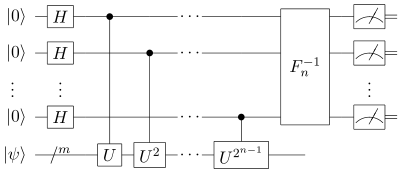
\includegraphics[scale=.6]{imagens/circex.png}
%\caption{Representação do Algoritmo de Shor} 
%\label{fig:circex}
%\end{figure}



\section{Modelo qGM}
Provê uma nova abordagem para modelagem de algoritmos quânticos, substituindo a noção de portas quânticas pelo conceito de processos elementares (PEs) \cite{Schmalfuss14}.

Fundamenta-se na teoria dos espaços coerentes, apresentados por Girard. Os objetos do espaço do domínio $\mathbb{D}_\infty$ são relevantes por definirem conjuntos coerentes que interpretam processos quânticos possivelmente infinitos, rotulados por pontos de espaço geomátrico, os quais caracterizam a base computacional para os conjuntos de vetores e matrizes de dimensões $n$ do espaço de Hilbert $\mathbb{H}$ \cite{maron:2013:ccgrid}.

Logo, podemos definir que,  um processo quântico é o resultado da sincronização de PEs que descrevem por completo uma transformação quântica. No decorrer da simulação ocorre a execução simultânea dos Pes, manipulando dados no espaço de memória de forma análoga à aplicação da transformação da porta $H$ sobre o vetor estado do sistema, simulando assim, o comportamento do sistema. A existência de processos quânticos parciais se dá a partir da aplicação parcial de uma transformação quântica devido a existência de indefinições acerca de determinados conjuntos de vetores cujos valores ainda não são conhecidos \cite{maron:2013:ccgrid}. 

A computação é realizada através de uma transição de estados associados a uma localização espacial obtida a partir da sincronização de processos clássicos, o que caracteriza a unidade de tempo computacional. Através da representação parcial associada sobre a evolução do estado de um sistema quãntico. No ambiente VPE-qGM um PE é um elemento fundalmentamente estruturado pelos atributos \cite{MARON12b}13 \cite{Schmalfuss14}.

\begin{enumerate}
    \item Ação: Corresponde à função atribuída ao PE, composta por transformações quãnticas sincronizadas. Isto é, transformações aplicadas a diferentes qubits em um mesmo instante de tempo.
    \item Parâmetros: Agregam dados auxiliares associados às definições das transformações quãnticas.
    \item Posição: Posição de escrita em um espaço de endereçamento global e compartilhado para armazenar o resultado calculado pelo PE.
\end{enumerate}

Nesse padrão de memória global compartilhada, ocorre a modelagem do espaço de estados quãnticos do sistema, onde cada posição e seu valor de armazenamento correspondem respectivamente a um estado e a probabilidade de ocorrência associada a ele (amplitude) \cite{Schmalfuss14}.

A relação entre memória e processo se dá pela seguinte forma: um PE pode ler de vários estados representados na memória, porém, só pode escrever em uma posição dela. A fim de exemplificar, considere uma aplicação de $(H|\psi\rangle)$, ao realizar essa operação verifica-se a ocorrência de duas atribuições clássicas simultâneas \cite{maron:2013:ccgrid}:

\begin{enumerate}
    \item somatório das amplitudes, associando o resultado, acrescido do valor de normalização $\frac{1}{\sqrt{2}}$ ao estado $|0\rangle$.
    \item subtração das amplitudes, associando o resultado, acrescido do valor de normalização $\frac{1}{\sqrt{2}}$ ao estado $|1\rangle$
\end{enumerate}

A abordagem qGM especifica que 1 ou 2 são representados por dois PEs sincronizados cujos atributos estabelecem um comportamento análogo aos vetores componentes que modelam a matriz associada a correspondente transformação quântica. Portanto, no decorrer da simulação ocorre a execução simutânea dos Pes no espaço de memória realizando uma operação equivalente a aplicação $H$, emulando assim, o comportamento de sistemas quânticos \cite{Schmalfuss14}.



\subsection{Ambiente VPE-qGM}

É um ambiente, que tem por objetivo prover a modelagem e simulação de algoritmos quânticos considerando o modelo qGM. Os seus principais componentes estruturais são \cite{maron:2013:ccgrid}:

\begin{itemize}
    \item $qGM$ (Quantum Process Editor): IDE para o desenvolvimento gŕafico dos algoritmos, modelados através da aplicação de uma série de constutores;
    
    \item $qME$ (Quantum Memory Editor): Interface para definição do estado inicial do sistema quântico. Um grid de memória armazena cada estado básico e a correspondente modelando um vetor de estado. Permite a configuração da memória de maneira simplificada abstraindo conceitos complexos vinculados ao espaço de estados do sistema; 
    
    \item $qS$ (Quantum Simulator): A partir das estruturas definidas nas interfaces do qPe e qME, o qS realiza a simulação do algoritmo quântico, suportando duas abordagens: simulação passo-a-passo e distribuída. Simula a partir de arquivos descritores de processos de memória;
    
    \item $qGM-Analyzer$: Biblioteca para realização das computações associadas aos componentes cada passo do algoritmo quântico, estando integrada à interface qS. O suporte para aceleração por GPU é estabelecido nesta biblioteca.
    
\end{itemize}

O ambiente possibilita executar as simulações em dois modos, total e passo-a-passo, permitindo desse modo um total controle sobre a simulação \cite{MARON10}.



\chapter{Medidas Quânticas}
%explicar um pouco melhor a importancia da medida
Foi postulado que sistema quânticos fechados evoluem de acordo com transformações unitárias. Medições são importantes pois são a partir delas que obtemos as informações dos circuitos quânticos quando os mesmos são simulados. Esse capítulo irá tratar dos tipos de medições que podem ser feitas em um circuito quântico e as suas propriedades.

%medida%%%%%%%%%%%%%%%%%%%%%%%%%%%%%%%%%%%%%%%%%%%%%%%%%%%%%%%%%%%%%%%%%
\section{Medida projetiva}
%tentar explicar como a medida funciona, talvez fazer uma árvore de execução, com um exemplo ( 1/sqrt(3) 
O processo de medida, na linguagem do espaço de Hilbert, é ser descrito como um processo de filtração representado por um operador de projeção $P_m$ associado a um observável M, junto com seu auto-valor $M_m$ e seu auto estado $|\psi\rangle$. A projeção extrai o componente do estado quântico que aponta na direção de $|\psi\rangle$:

\begin{equation}O 
    P_m|\psi\rangle= P_m\sum\limits_{i}\alpha_i|\psi_i\rangle
\end{equation}

Depois que a medida foi efetuada o sistema permanece no estado $|\psi_m\rangle$.
A probabilidade de encontrar o estado $|\psi_\rangle$ no estado $|\psi_m\rangle$ é:
\begin{equation}
    \langle\psi|P_m|\psi\rangle= \langle\psi|\alpha_m|\psi_m\rangle 
    =\sum\limits_{i}\alpha_i^*|\psi_i\rangle
    =\alpha_m^*\alpha_m\langle\psi_m|\psi_m\rangle
    =\alpha_m^*\alpha_m=P_m
\end{equation}

É importante dizer também que as projeções associadas com os auto-valores de $M$ são Hermitianas. Logo, estas projeções são ortogonais e somam 1.
\begin{equation}
    \sum\limits_{i}P_i=1
\end{equation}
Então, o estado após a medida deve ser 
\begin{equation}
    |\psi_m\rangle= \frac{1}{\alpha_m}P_m|\psi\rangle =
    \frac{P_m|\psi\rangle}{\sqrt{\langle\psi|P_m|\psi\rangle}}
\end{equation}


No exemplo, cada um dos ramos da árvore separa as medições, à esquerda se o qubit medido for $|0\rangle$ e à direita se for $|1\rangle$ . Após feita a primeira medição, obtém-se um estado normalizado para cada ramo, cada um deles contendo a sua probabilidade de ocorrência. Após isso, de forma análoga, ocorre outra medição onde cada estado normalizado gera dois novos estados.


\begin{center}
    
%arvore do exemplo
\begin{forest}
  [$\frac{1}{\sqrt{30}} (|00\rangle +2|01\rangle +3|10\rangle + 4|11\rangle)$
    [$\text{p_0=} \frac{1}{6}$
     [$\frac{1}{\sqrt{5}}(|00\rangle+|01\rangle$
       [$\text{p=}\frac{1}{5}$
          [$|00\rangle$
             [$\text{p_{00}=}\frac{1}{30}$]
          ]
       ]

       [$\text{p=}\frac{4}{5}$
          [$|01\rangle$
             [$\text{p_{01}=}\frac{4}{30}$]
          ]
       ]
     ]
       
    ]
    [$\text{p_1=}\frac{5}{6}$
        [$\frac{1}{5}(3|10\rangle+4|11\rangle$
        [$\text{p=}\frac{9}{25}$
           [$|10\rangle$
              [$\text{p_{10}=}\frac{9}{30}$]
           ]
        ]
        [$\text{p=}\frac{16}{25}$
           [$|11\rangle$
              [$\text{p_{11}=}\frac{16}{30}$]
           ]
        ]
        ]
       
    ]
  
  ]
\end{forest}
\end{center}

%É importante ressaltar que, neste exemplo a medida foi feita %levando em consideração a probabilidade obtenção do primeiro qubit %ser $|0\rangle$. Após a primeira medição, o estado obtido foi %$\frac{1}{\sqrt{5}}(|00\rangle+|01\rangle$ se o qubit medido foi %$|0\rangle$, com $\frac{1}{\sqrt{6}}$ de probabilidade. Se o %primeiro qubit encontrado após a primeira medida for $|1\rangle$, %então teremos o estado $\frac{1}{5}(3|10\rangle+4|11\rangle$, com %$\frac{5}{\sqrt{6}}$ de probabilidade.


A probabilidade da medida resultante do primeiro qubit ser 0 foi de $ \frac{1}{\sqrt{5}} (|00\rangle +2|01\rangle$) com $P=\frac{1}{6}$ e do segundo qubit também ser 0 foi de $P=\frac{1}{5}$, resultando então em $P=\frac{1}{30}$ a probabilidade de se obter o estado $|00\rangle$.

A probabilidade de se obter 0 na primeira medição e 1 na segunda foi de $P=\frac{1}{6}$ e $P=\frac{4}{5}$, resultando em $P=\frac{4}{30}$ a probabilidade de se obter o estado $|01\rangle$.  
A probabilidade de se obter 1 na primeira medição e  na segunda foi de $P=\frac{9}{25}$ e $P=\frac{4}{5}$ respectivamente, resultando em $P=\frac{9}{30}$ a probabilidade de se obter o estado $|10\rangle$. 

A probabilidade de se obter 1 na primeira medição e 1 na segunda foi de $P=\frac{16}{25}$ e $P=\frac{16}{30}$, resultando em $P=\frac{4}{30}$ a probabilidade de se obter o estado $|11\rangle$. 


\section{Na base de Bell}

A base de Bell combina de forma não-trivial todos os conceitos básicos da Mecânica Quântica. Desse modo, é um exemplo ideal para demonstração de processamento que pode ser realizado pela Mecânica quântica.

Para tal demonstração, vamos utilizar dois parceiros, "Alice" e "Bob", que se encontram separados por uma grande distância do outro. O objetivo é transmitir informação clássica de Alice para Bob. Então, se Alice quiser enviar dois bits clássicos para Bob utilizando um único qubit, tanto Alice quanto Bob devem estar inicialmente estar emaranhados:
\begin{equation}
    |\psi\rangle = \frac{|00\rangle+|11\rangle}{\sqrt{2}}
\end{equation}

Note que o primeiro qubit se encontra com Alice e o segundo com Bob e $|\psi\rangle$ foi  pré-fixado. Ao enviar o seu qubit para Bob é possível para Alice comunicar dois bits de informação clássica, adotando o seguinte procedimento: se ela quiser enviar a sequência "00", não deve fazer nada com o seu qubit. Se ela deseja enviar a sequência "01", deve aplicar uma porta X em seu qubit. E finalmente, se ela quiser enviar "11", deve aplicar a porta $i$Y ao seu qubit. Os quatro estados resultantes são:

\begin{equation}
    00: |\psi\rangle \rightarrow \frac{|00\rangle+|11\rangle}{\sqrt{2}}
\end{equation}

\begin{equation}
   01: |\psi\rangle \rightarrow \frac{|00\rangle-|11\rangle}{\sqrt{2}}
\end{equation}

\begin{equation}
    10: |\psi\rangle \rightarrow \frac{|10\rangle+|01\rangle}{\sqrt{2}}
\end{equation}

\begin{equation}    
    11: |\psi\rangle \rightarrow \frac{|01\rangle-|10\rangle}{\sqrt{2}}
\end{equation}
    
Esses quatro estados são conhecidos como \textit{base de Bell}, e podem ser distinguidos por meio de uma medida apropriada. Se Alice enviar o seu qubit para Bob, uma vez de posse dos dois qubits, ele pode realizar uma medida na base de Bell e determinar qual dentre as quatro sequencias Alice enviou.

Assim, manipulando apenas um qubit, Alice é capaz de enviar dois bits de informação clássica, mesmo os dois qubits estando envolvidos no protocolo, mas Alice nunca precisa interagir com o segundo.\cite{chuang00a}

\section{Resistente a falhas}
%pagina 530
Uma das aplicações mais poderosas da correção quântica de erro não é a mera proteção da informação quântica armazenada ou transmitida, mas a proteção da informação quãntica durante o processo \emph{dinâmico de computação}. É surpreendente, mas possível implementar a computação quântica de forma arbitrariamente boa, mesmo com portas lógicas defeituosas, desde que a probabilidade de erro por porta esteja abaixo de um certo \emph{limiar resistente a falhas} que são usadas para chegar a esse resultado. \cite{chuang00a}.


Uma ferramenta extremamente importante na construção de circuitos resistentes a falhas é a capacidade de \textit{ medir um operador M}. As medidas são usadas para codificar, ler os resultados da computação, diagnosticar a síndrome nas correções de erro e preparar estados auxiliares para a construção das portas $\frac{\pi}{8}$ e Toffoli. Consequentemente, são cruciais para a computação quântica resistente a falhas. Para que um procedimento de medida codificada seja resistente a falhas, requer-se que duas coisas ocorram para se prevenir a propagação de erros. Primeira: uma única falha em qualquer etapa do procedimento deve ocasionar no máximo um erro em qualquer um dos blocos de qubits ao final do procedimento. Segunda: mesmo que uma única falha ocorra durante o procedimento, requer-se que o resultado da medida esteja correto com a probabilidade 1-$O(p^2$). Esse último requisito é extremamente importante, pois o resultado da medida pode ser usado para controlar outras operações no computador quântico e, se ela estiver incorreta, o erro pode se propagar, afetando muitos qubits em blocos de qubits codificados. 

Suponha que se possa dar uma representação codificada transversal para um observável M em um código quântico, como uma aplicação de uma porta M' bit a bit a cada qubit do código. Por exemplo, para o código de Steane, M = H terá uma implementação transversal como aplicação bit a bit de M'=H, ao passo que a implementação transversal de M=S utiliza a aplicação binária M'= ZS. Isso sugere um possível circuito para a medida de M codificado nos dados codificados, mas como o código de Steane, precisaria de mais qubits. 

\begin{figure}
    \centering
    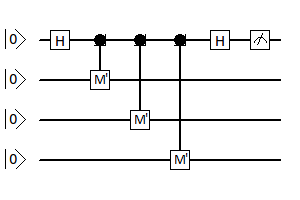
\includegraphics[width=.5\textwidth]{imagens/ExemplodeResistenciaqueNaoF.png}
    \caption{Esquema para realização de uma medida em um observável codificado M com implementação transversal como aplicação bit a bit de M'. O circuito não é resistente a falhas.}
    \label{fig:falhas}
\end{figure}

Infelizmente, esse circuito não é resistente a falhas, pois o erro se propagará adiante e afetará todos o qubits codificados.




Para se ter um circuito resistente a falhas, se introduz um qubit auxiliar, inicialmente no estado $|0\rangle$, para cada qubit de dado. A ideia básica é que, para se verificar o estado do gato, é suficiente mostrar que uma medida $Z_iZ_j$ para todos os pares de qubits $i$ e $j$ no estado do gato terá 1 como resultado. Ou seja, a paridade de qualquer par de qubits no estado gato é par. Para verificar isso em um par particular $Z_i Z_j$ ($Z_2 Z_3$, por exemplo), introduz-se um qubit extra, inicializado em $|0\rangle$. Computa-se a paridade de dois dos qubits no sistema auxiliar por meio de duas portas CNOT tendo os qubits auxiliares como controles e o qubit extra como alvo, antes da medida do qubit extra. Se a paridade medida for igual a 1, saberemos que o qubit auxiliar não está no estado de gato. Nesse caso, ele é descartado e o processo reinicia. 

O procedimento não é resistente a falhas, pois é fácil mostrar que existem falhas de componentes individuais que levam a mais de uma mudança de fase no estado auxiliar. Por exemplo, se ocorrer um erro | no qubit extra entre as portas CNOT, ele pode se propagar, causando erros Z em dois qubits auxiliares. Felizmente, é fácil mostrar que múltiplos erros Z nos qubits auxiliares $não$ se propagam para os dados codificados, embora eles possam causar erros na leitura da medida final. 
\begin{figure}[ht!]
    \centering
    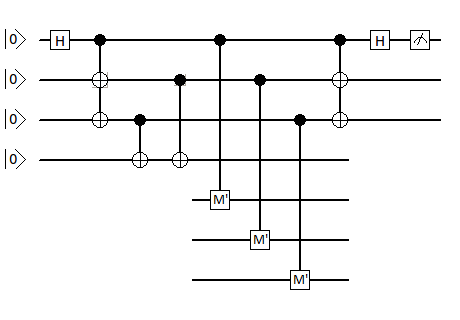
\includegraphics[width=.6\textwidth]{imagens/resistenteafalhas.png}
    \caption{Procedimento esquemático para uma medida resistente a falhas de um observável M sobre dados codificados.}
    \label{fig:falhas}
\end{figure}


Assim, a probabilidade de que a medida esteja errada duas ou mais vezes será no máximo O$(p^2)$, onde $p$ é a probabilidade de falha de uma única componente. Os erros X e Y $podem$ se propagar causar erros nos dados codificados, porém, uma falha durante a preparação do estado do gato e o procedimento de verificação pode causar no máximo um erro Z ou Y no sistema auxiliar após a verificaçãoe portanto no máximo um erro nos dados codificados, garantindo a resistência a falhas. 

Após a verificação do estado do gato, portas $M'$-controladas são implementadas entre pares de qubits do sistema auxiliar dos dados, sendo que nenhum qubit auxiliar é usado mais de uma vez. Logo, se o sistema auxiliar estiver no estado $|oo...o\rangle$, nada ocorrerá com os dados codificados, mas, se o estado auxiliar for $|11...1\rangle$, a operação $M$ codificada é aplicada aos dados. É o estado do gato que assegura que os erros não se propagarão de uma porta $M'$-controlada para outra, e portanto um único erro no estágio de verificação resulta em no máximo um erro nos dados codificados. Por fim, o resultado da medida é obtido decodificando o estado do gato com uma série de portas CNOT e uma Hadamard. O qubit resultante será 0 ou 1, dependendo do autovalor do estado dos dados \cite{chuang00a}. 


\section{No formalismo de estabilizadores}
A ideia central do formalismo de estabilizadores pode ser ilustrada pelo estado EPR de dois qubits:
\begin{equation}
    |\psi\rangle=\frac{|00\rangle+|11\rangle}{\sqrt{2}}
\end{equation}

Esse estado satisfaz as identidades $X_1 X_2|\psi\rangle = |\psi\rangle$ e $Z_1Z_2|\psi\rangle = |\psi\rangle$, pois o estado $|\psi\rangle$ é estabilizado pelos operadores $X_1 X_2$ e $Z_1Z_2$, também é preciso dizer que esse estado quântido é o \textit{único} estado estabilizado por esses operadores. A ideia básica do formalismo de operadores é que muitos estados quânticos podem ser mais facilmente descritos trabalhando-se com os operadores que os estabilizam, do que com os estados propriamente ditos. Ocorre que muitos códigos quãnticos (incluindo o CSS e o código de Shor) podem ser descritos de forma muito mais compacta utilizando-se os estabilizadores em vez dos vetores de estado. Mais importante ainda, erros em qubits e em operações tais como a porta Hadamard, porta de fase, e mesmo a porta CNOT e medidas na base computacional podem ser descritas através do formalismo de estabilizadores.

%PEGAR APÊNDICE, PÁGINA 655
O formalismo de estabilizadores funciona através de uma aplicação inteligente da \textit{teoria dos grupos} \cite{olson1999logica}.  O grupo mais importante é o \textit{grupo de Pauli $G_n$}, sobre $n$ qubits. Para um único qubit, o grupo de Pauli consiste em todas as matrizes de Pauli, junto com fatores multiplicativos $\pm1$ e $\pm i$:

\begin{equation}
    G1 \equiv \{ \pm I, \pm iI, \pm X, \pm X, \pm Y, \pm Y, \pm Z, \pm iZ \}
\end{equation}

Esse conjunto de matrizes forma um grupo sob a operação de multiplicação matricial. Pode-se perguntar por que não omitir os fatores multiplicativos $\pm 1$ e $\pm i$; a razão de sua inclusão é que eles garantem que $G_1$ seja fechado sob multiplicação, e portante forme um grupo legítimo. O grupo de Pauli geral, de $n$ qubits, é definido como todas as matrizes formadas pelos produtos tensoriais de ordem $n$ das matrizes de Pauli, com os fatores $\pm 1$ e $\pm i$ inclusos. 

Seja $S$ um subgrupo de $G_n$. $VS$ é definido como o conjunto dos estados de n qubits fixos para cada elemento de $S$. $VS$ é o \textit{espaço vetorial estabilizado} por $S$; diz-se que $S$ é o estabilizador do estado $VS$, na medida em que cada elemento de $VS$ é estável sob a ação dos elementos em $S$  \cite{chuang00a}.



\section{Medida POVM}
O postulado 3 envolve dois elementos. Primeiro, fornece uma regra que descreve a estatística de medidas, ou seja, as diversas possibilidades dos diferentes resultados. Segundo, diz qual o estado do sistema após a medida. Contudo, em algumas aplicações, o estado do sistema após a medida é de pouco interesse, sendo mais importante a probabilidade dos diferentes resultados da medida. Esse é, por exemplo, o caso em que a medida é feita somente uma vez, e o experimento é concluído. Para esses casos, existe uma ferramenta matemática conhecida como \emph{formalismo POVM}(Positive Operator-Valued Measure), que é especialmente bem adaptado para a análise de medidas. Esse formalismo é uma consequência simples da descrição geral de medidas introduzidas no postulado 3. 
Imagine que uma medida descrita por operadores $M_m$ seja realizada em um sistema quântico no estado $|\psi\rangle$. A probabilidade de o resultado ser m é dada por $p(m) =\langle \psi|M^\dagger _m M_m|\psi\rangle$. Seja a definição: 
\begin{equation}
    E_m\equiv M^\dagger_mM_m.
\end{equation}

Então, $E_m$ é um operador positivo tal que $\sum_m E_m = I$ e p(m) $= \langle|E_m|\psi\rangle$. Logo, o conjunto de operadores $E_m$ é suficiente para determinar as probabilidades dos diferentes resultados das medidas. Os operadores $E_m$ são conhecidos como \emph{elementos POVM} associados à medida. O conjunto completo $E_m$ é conhecido como um $POVM$. 

Como exemplo POVM, considere uma medida projetiva com operadores $P_m$, em que $P_m$ são projetores tais que $P_mP_m' = \delta _m,_m'P_m$ e $\sum_mP_m=I$. Nesse caso( e somente nesse caso) todos os elementos $POVM$ são idênticos aos operadores de medida, pois $E_m \equal P^\dagger_m P_m = P_m$ \cite{chuang00a}.

\chapter{Conclusão}




% Bibliografia http://liinwww.ira.uka.de/bibliography/index.html um
% site que cataloga no formato bibtex a bibliografia em computacao
% \bibliography{nomedoarquivo.bib} (sem extensao)
% \bibliographystyle{formato.bst} (sem extensao)

\bibliography{bibliografia} 
\bibliographystyle{abnt}
%\bibliographystyle{plain}

% Anexos (Opcional)
%\annex

%\chapter{Outro Anexo}


% Faz a capa do CDROM
\makecover

\end{document}

